%%%%%%%%%%%%%%%%%%%%%%%%%%%%%%%%%%%%%%%%%%
% Masters/Doctoral Thesis 
% LaTeX Template
% Version 1.43 (17/5/14)
%
% This template has been downloaded from:
% http://www.LaTeXTemplates.com
%
% Original authors:
% Steven Gunn 
% http://users.ecs.soton.ac.uk/srg/softwaretools/document/templates/
% and
% Sunil Patel
% http://ww% CC BY-NC-SA 3.0 (http://creativecommons.org/licenses/by-nc-sa/3.0/)
%
% Note:
% Make sure to edit document variables in the Thesis.cls file
%
%%%%%%%%%%%%%%%%%%%%%%%%%%%%%%%%%%%%%%%%%

%----------------------------------------------------------------------------------------
%	PACKAGES AND OTHER DOCUMENT CONFIGURATIONS
%----------------------------------------------------------------------------------------

\documentclass[11pt, oneside]{Thesis} % The default font size and one-sided printing (no margin offsets)

\graphicspath{{Pictures/}} % Specifies the directory where pictures are stored
\usepackage{siunitx}
\usepackage{xr}

\usepackage{subfig}
%\usepackage[square, numbers, comma, sort&compress]{natbib} % Use the natbib reference package - read up on this to edit the reference style; if you want text (e.g. Smith et al., 2012) for the in-text references (instead of numbers), remove 'numbers' 
\hypersetup{urlcolor=blue, colorlinks=true} % Colors hyperlinks in blue - change to black if annoying
\title{\ttitle} % Defines the thesis title - don't touch this

\begin{document}

\frontmatter % Use roman page numbering style (i, ii, iii, iv...) for the pre-content pages

\setstretch{1.3} % Line spacing of 1.3

% Define the page headers using the FancyHdr package and set up for one-sided printing
\fancyhead{} % Clears all page headers and footers
\rhead{\thepage} % Sets the right side header to show the page number
\lhead{} % Clears the left side page header
\pagestyle{fancy} % Finally, use the "fancy" page style to implement the FancyHdr headers

\newcommand{\HRule}{\rule{\linewidth}{0.5mm}} % New command to make the lines in the title page

% PDF meta-data
\hypersetup{pdftitle={\ttitle}}
\hypersetup{pdfsubject=\subjectname}
\hypersetup{pdfauthor=\authornames}
\hypersetup{pdfkeywords=\keywordnames}

%----------------------------------------------------------------------------------------
%	TITLE PAGE
%----------------------------------------------------------------------------------------

\begin{titlepage}
\begin{center}

\textsc{\Large A thesis submitted to the University of Manchester for the degree
of Doctor of Philosophy in the Faculty of Science and Engineering}\\[0.5cm] % Thesis type

\HRule \\[0.4cm] % Horizontal line
{\huge \bfseries \ttitle}\\[0.4cm] % Thesis title
\HRule \\[1.5cm] % Horizontal line
 %g
\begin{minipage}{0.4\textwidth}
\begin{flushleft} \large
\emph{Author:}\\
{\authornames} % Author name - remove the \href bracket to remove the link
\end{flushleft}
\end{minipage}
\begin{minipage}{0.4\textwidth}
\begin{flushright} \large
\emph{Supervisor:} \\
{\supname} % Supervisor name - remove the \href bracket to remove the link  
\end{flushright}
\end{minipage}\\[3cm]
 
\large 
\groupname\\\deptname\\\univname\\[2cm] % Research group name and department name

{\large \today}\\[4cm] % Date

\includegraphics[scale=0.35]{logo} % University/department logo - uncomment to place it
 
\vfill
\end{center}

\end{titlepage}


%----------------------------------------------------------------------------------------
%	LIST OF CONTENTS/FIGURES/TABLES PAGES
%----------------------------------------------------------------------------------------

\pagestyle{fancy} % The page style headers have been "empty" all this time, now use the "fancy" headers as defined before to bring them back

\lhead{\emph{Contents}} % Set the left side page header to "Contents"
\tableofcontents % Write out the Table of Contents

\lhead{\emph{List of Figures}} % Set the left side page header to "List of Figures"
\listoffigures % Write out the List of Figures

%\lhead{\emph{List of Tables}} % Set the left side page header to "List of Tables"
%\listoftables % Write out the List of Tables


%----------------------------------------------------------------------------------------
%	THESIS CONTENT - CHAPTERS
%----------------------------------------------------------------------------------------

\mainmatter % Begin numeric (1,2,3...) page numbering

\pagestyle{fancy} % Return the page headers back to the "fancy" style

% Include the chapters of the thesis as separate files from the Chapters folder
% Uncomment the lines as you write the chapters

%input{Chapters/Chapter1}
%input{Chapters/Chapter2} 
%% Chapter Template

\chapter{Direct Reactions} % Main chapter title

\label{Chapter3} % Change X to a consecutive number; for referencing this chapter elsewhere, use \ref{ChapterX}

\lhead{Chapter 3. \emph{Direct Reactions}} % Change X to a consecutive number; this is for the header on each page - perhaps a shortened title


\section{Introduction}

Direct reactions are a way to probe nuclear structure. As the name suggests, they are one-step processes, where one reaction happens in a collision between a target and projectile nucleus. The alternative to a direct reaction is a compound reaction, where one or more intermediate states are created between the initial and final state.

Direct reactions are more likely to happen in a glancing collision, i.e. the impact parameter of the collision is approximately equal to the nuclear radius. This is because the more time the projectile spends in or near the target, the more likely it will undergo multiple reactions. Because of the glancing nature of the collision, there is a smaller exchange of energy, and reaction products are scattered at forward angles to the beam. For comparison, in compound reactions, reaction products are emitted isotropically in the centre of mass frame, and are more likely to happen in collisions with small impact parameters.

Direct reactions are denoted by A(a,b)B, where A and B are the target and recoil nuclei, and a and b are the projectile and ejectile nuclei. A and a are referred to as the incoming partition together denoted by $\alpha$, and B and b are the outgoing partition, denoted by $\beta$.

This work discusses single nucleon transfer reactions (p,d) and (d,p) on neutrinoless double-beta decay candidate nuclei. Single nucleon transfer is useful to probe single particle structure, due to the excitation of only a single degree of freedom. The probability of a single nucleon transfer reaction occuring is given by Fermi's Golden rule,

\begin{equation}
\lambda = \frac{2 \pi}{\hbar} |V_{\beta \alpha}| \rho_{E_k}\mathrm{,}
\end{equation}

where $\rho_{E_k}$ is the density of final states, and $|V_{\beta \alpha}|$ is the matrix element for the transition, which depends on the overlap between initial and final states.

\subsection{DWBA} \label{ssec:DWBA}

The distorted-wave Born approximation (DWBA) is a model of scattering theory, and is the one that has been used to calculate cross-sections in this study. For a full derivation of DWBA, see Refs. \cite{satchler,glendenning}.

The starting point is to consider the general cross-section for a reaction, 

\begin{equation}
\bigg ( \frac{\mathrm{d} \sigma}{\mathrm{d} \Omega} \bigg )_{\beta \alpha} = \frac{\mu_\alpha \mu_\beta}{(2 \pi \hbar)^2}  \frac{k_\alpha}{k_\beta} \mathit{T}_{\beta\alpha}^2\mathrm{,}
\end{equation}

where $k$ are the wavenumbers, representing the momenta, and $\mu$ are the reduced masses. $\mathit{T}_{\beta\alpha}$ is the transition matrix element for the reaction. This equation is related to Fermi's Golden Rule.

\begin{equation}
\mathit{T}_{\beta\alpha} =  \langle \Psi_\beta | V | \Psi_\alpha \rangle,
\end{equation}

where $\Psi_{\alpha, \beta}$ are the total wavefunctions for the partitions $\alpha$ and $\beta$. $V$ is the interaction potential.

Initially, these $\Psi$ were modelled as plane waves. This reproduced the changing of the peak of the angular distribution of cross-sections with angle, but failed to reproduce the cross-sections accurately. In actuality, the potentials are distorted by the interaction with the target.

The Born approximation is the treatment of the interaction between two nucleons being dominated by elastic scattering. Any other reaction removes flux from the outgoing elastic scattering channel. This is modelled using complex potentials, and is the application of first-order pertubation theory to scattering.

For the DWBA approach, we begin by considering the wavefunction of internal states in a partition. For the (d,p) reaction we consider $\psi_\alpha$. This is separable such that

\begin{equation} \label{eq:separable}
\psi_\alpha = \psi_d(x_d) \psi_T(x_T)\mathrm{,}
\end{equation}

where $d$ pertains to the deuteron, $T$ pertains to the target, and $x$ are the internal co-ordinates.

The total Hamiltonian $H$ can be separated into these internal co-ordinates, and the relative co-ordinates for the partition, such that

\begin{equation} \label{eq:hamiltonian}
H = H_\alpha + T_\alpha + V_\alpha\mathrm{,}
\end{equation}

where $H_\alpha$ is the internal Hamiltonian, $T_\alpha$ is the relative kinetic energy, and $V_\alpha$ is the interaction potential. 

Similarly to modelling the shell model, an auxillary potential $U_\alpha$ is introduced, so that

\begin{equation} \label{eq:residual}
H = H_\alpha + T_\alpha + (V_\alpha - U_\alpha) + U_\alpha \mathrm{.}
\end{equation}

$U_\alpha$ is chosen to replicate elastic scattering, which leaves $V = V_\alpha - U_\alpha$ as an imaginary potential which removes flux from the elastic channel. Equations~\ref{eq:separable},~\ref{eq:hamiltonian}~and~\ref{eq:residual} can be found for the $\beta$ channel also.

$V_\beta$ is the sum of the reaction of the outgoing proton with the target, and with the neutron. $U_\beta \approx V_{pT}$, so $V \approx V_{pn}$, where $V_{pt}$ and $V_{pn}$ are the interactions between the proton and target and proton and deuteron respectively.

The total wavefunctions can be separated into a product of the internal and relative motion,

\begin{equation}
\Psi_{\alpha,\beta} = \psi_{\alpha,\beta}\chi_{\alpha,\beta}\mathrm{,}
\end{equation}

where $\chi_{\alpha,\beta}$ are distorted waves which are the solution to the homogeneous Schr{\"o}dinger equation

\begin{equation}
(H_{\alpha,\beta}-T_{\alpha,\beta}-V_{\alpha,\beta})\chi_{\alpha,\beta} = 0
\end{equation} 

The transition matrix element then becomes

\begin{equation}
\mathit{T}_{\beta\alpha} =  \langle \psi_R \psi_p \chi_\beta | V_{pn} | \psi_T \psi_d \chi_\alpha   \rangle\mathrm{,}
\end{equation}

where $R$ pertains to the residual nucleus.

The wavefunction of the residual nucleus is equivalent to the wavefunction of the target with an extra neutron in a superposition of single-particle orbits,

\begin{equation}
\psi_R = \sum_{njl} \gamma_{njl} \phi_{njl} \psi_T \mathrm{,}
\end{equation}

where $\gamma_{njl}$ are probability amplitudes, $\phi_{njl}$ are the single-particle wavefunctions, and the sum is over the single-particle quantum numbers $n,j,l$. The deuteron with wavefunction $\psi_d$ is similarly a proton with a neutron orbiting in a different configuration of single-particle states $\sum_{n'j'l'}\phi_{n'j'l'}$.

With this, the differential cross section is then

\begin{equation}
\bigg ( \frac{\mathrm{d} \sigma}{\mathrm{d} \Omega} \bigg )_{\beta \alpha} =\frac{\mu_\alpha \mu_\beta}{(2 \pi \hbar)^2}  \frac{k_\alpha}{k_\beta}  \sum_{njl} \sum_{n'j'l'} \gamma_{njl}^2\gamma_{n'j'l'}^2 |\langle  \phi_{njl} \chi_\beta | V_{pn} | \phi_{n'j'l'} \chi_\alpha  \rangle |^2\mathrm{.}
\end{equation}

For (d,p) and (p,d), $\gamma_{n'j'l'}$ is unity, because the deuteron only has one bound state. For other reactions this needs to be treated in more detail.  $\gamma_{njl}^2$ is the probability of finding the neutron in a particular single particle state in the residual nucleus, and is also known as the spectroscopic factor. Henceforth, the differential cross-section in the case where $\gamma_{n'j'l'}$ is unity will be referred to as the DWBA cross-section.

\subsection{Optical Model} \label{ssec:opticalModel}


To model $V$ and $U$, the optical model was used. The optical model treats the target nucleus similarly to a lens to the "light" ray of the beam. It absorbs some of the beam, scatters some, and transmits some. Optical models describe elastic scattering, because it is the dominant scattering channel at energies used in transfer reaction studies. However, corrections must be applied to account for scattering into inelastic channels.

The optical model potential employs a mean-field potential similar to a shell model. The form of this mean field potential is a Woods-Saxon $f(r)$ with a spin-orbit term. This has an imaginary component to account for the flux out of the elastic channel. There is also an imaginary surface term to account for  low-level collective excitations. As well as the nuclear potential, the Coulomb potential $V_C(r)$ is also considered.

The general expression for the total optical model potential is

\begin{equation}
\begin{split}
V(r) = \bigg [ V_C(r) - V_rf(r) + V_{so}\frac{1}{r}\frac{\partial f(r)}{\partial r}({\bf \hat{L} \cdot \hat{S}}) \bigg ] \\
	+ i \bigg [ -W_rf(r) + W_{so}\frac{1}{r}\frac{\partial f(r)}{\partial r}({\bf \hat{L} \cdot \hat{S}}) + 4W_s \frac{\partial f(r)}{\partial r} \bigg ] \mathrm{,}
\end{split}
\end{equation}

where coeffiecients $V_i$ and $W_i$ are the magnitudes of the potentials. The suffixes $i =  v, s, so$ stand for volume, surface, and spin-orbit respectively.

These coefficients, plus the diffuseness and radii, are the \textit{optical model parameters}. They are determined experimentally. This is done by measuring elastic scattering cross-sections over a range of nuclei and energies, and fitting  the optical model parameters to best fit the data.

This can be done over a small range of nuclides and energies for a local fit, or a large number for a global fit. Local fits sometimes only use one nuclide and energy. The advantages of using global paramaters is that the fit parameters are more reliable for a larger number of data points, and can be used for a large range of reactions and energies. The advantage of local parameters is that they may capture local fluctuations in parameters that may be smoothed over by a global fit. In this study, global parameters from a study by An and Cai\cite{ancai} were used for deuterons, and global parameters for protons from a study by K\"oning and Delaroche\cite{koningdelaroche} were used.


\subsection{Spectroscopic Factors and Occupancies}

The residual interactions fragment the single-particle strength across multiple excitation energies. However, the total single-particle strength can be recovered. This is done using spectroscopic factors and the \textit{Macfarlane and French sum rules}.

The spectroscopic factor is, as seen in section~\ref{ssec:DWBA}, a function which describes the overlap between the final state, and the target nucleus with a nucleon outside of it. It can be calculated experimentally by comparing the cross-section to a calculated cross-section assuming a pure single-particle state. Quantatively, this is

\begin{equation}
\bigg ( \frac{\mathrm{d} \sigma}{\mathrm{d} \Omega} \bigg )_{\mathrm{expt}} = C^2S \bigg ( \frac{\mathrm{d} \sigma}{\mathrm{d} \Omega} \bigg )_{\mathrm{DWBA}}\mathrm{,}
\end{equation}

where $S$ is the spectroscopic factor for the state and $C^2$ are isospin Clebsch-Gordan coefficients.

$C^2S$ can therefore be extracted by comparing the DWBA cross-section for a reaction to a state with the experimental cross-section. The cross-sections are $\ell$ dependent, so the $\ell$ for that state must be determined to obtain an accurate spectroscopic factor.

If all of the spectroscopic factors for a given total angular momentum $j$ are summed up, the occupancy (for removal reactions) or vacancy (for addition reactions) of the corresponding shell  can be deduced. These are the Macfarlane and French sum rules\cite{macfarlanefrench}. The occupancies are given by

\begin{equation}
\mathrm{Occupancy} = \sum_{i}C^2S_i^{(\mathrm{r})}\mathrm{,}
\end{equation}

where $S_i^{(\mathrm{r})}$ are the spectroscopic factors for each state in a removal reaction. The vacancies are given by

\begin{equation}
\mathrm{Vacancy} = \sum_{i}(2j+1)C^2S_i^{(\mathrm{a})}\mathrm{,}
\end{equation}

where this time $S_i^{(\mathrm{a})}$ are the spectroscopic factors for addition. The $(2j + 1)$ comes from the fact that neutrons can be added into any of the available states in the orbital. For a full orbital, the occupancy is $2j + 1$.
% Chapter Template

\chapter{Experimental Details} % Main chapter title
\graphicspath{{Pictures/}}
\label{Chapter4} % Change X to a consecutive number; for referencing this chapter elsewhere, use \ref{ChapterX}

\lhead{Chapter 4. \emph{Experimental Details}} % Change X to a consecutive number; this is for the header on each page - perhaps a shortened title

%----------------------------------------------------------------------------------------
%	SECTION 1
%----------------------------------------------------------------------------------------

\section{Introduction}

This section covers the experimental details of the measurements (d,p) and (p,d) transfer reactions on targets of \textsuperscript{116}Cd, \textsuperscript{114}Cd, and \textsuperscript{116}Sn. These measurements were made using the Q3D magnetic spectrometer located at the Maier-Leibnitz Laboratorium (MLL) in Munich. 

%----------------------------------------------------------------------------------------
%	SECTION 2
%----------------------------------------------------------------------------------------

\section{Experimental Procedure}


 ----------------------------------
%	SUBSECTION 1
%-----------------------------------
\subsection{Ion Source}
Proton and deuteron ion beams were produced in a Stern-Gerlach ion source\cite{sterngerlach}. This was operated without using the polarising Stern-Gerlach magnets, as no polarisation was needed for these measurements. This ion source used an electron cyclotron resonance (ECR) positive ion source, combined with a charge exchange cell. The charge exchange cell was required because the acccelerator required injection of negative ions due to the positive charge on the terminal used to produce the accelerating voltage.

The ECR ion source worked by applying a radio-frequency (RF) signal to a gas of the species of atom which was to be used as the beam. This was done in a constant magnetic field, so that the RF frequency matched the natural gyro-frequency of electrons in that magnetic field. This caused resonant acceleration in free electrons in the gas, which ionised the gas by colliding the resonant electrons with the gas atoms. These positive ions were then passed through a caesium jet in a charge exchange cell, which caused them to pick up two electrons and become negative ions.


\subsection{Tandem Accelerator}
The negative ions from the ion source were injected, via a \SI{150}{\kilo\volt} potential, into the MP tandem Van de Graaff accelerator. This accelerated the ions to \SI{15}{\mega\electronvolt} (deuterons) and \SI{22}{\mega\electronvolt} (protons). A central terminal of the accelerator was charged to a high voltage, which could reach approximately \SI{+15}{\mega\volt}\cite{highvoltage}. 

In the accelerator, negative ions were accelerated towards the central terminal by the electrostatic force. The terminal potential was maintained using pelletron chains. These consisted of a chain made of metal pellets connected by insulating nylon, rotating on two pulleys. One pulley was at the terminal, and the other situated by an inductor, which charged the pellets. After being charged, they transported positive charge to the terminal. Negative charge was transported away by the pellets on their return journey. A carbon stripper foil was placed in the central terminal, such that the beam ions lost their electrons upon passing through it. The newly positive beam ions were consequently accelerated away from the terminal with the same voltage. The energy of the beam $E_{\mathrm{beam}}$ was therefore

\begin{equation}
E_{\mathrm{beam}} = (|q_1| + |q_2|)V\mathrm{,}
\end{equation}

where $|q_1|$ and $|q_2|$ are the magnitude of the charges of the beam ions before and after being stripped of electrons, and $V$ is the terminal voltage. In this experiment, hydrogen beams were used so the beam energy was equal to $2V$, since the beam particles had $-1$ charge before and $+1$ charge after passing through the stripper foil. In this experiment, the voltage was held at \SI{7.5}{\mega\volt} for deuterons, \SI{11}{\mega\volt} for protons, and \SI{4.5}{\mega\volt} for elastic scattering measurements.

A diagram of the tandem accelerator is shown in Figure~\ref{tandemDiagram}. The relative positions of the beam line, terminal, and pelletron chains are shown.

\begin{figure}[h]	
\hspace*{-0.5cm}
\begin{center}	
	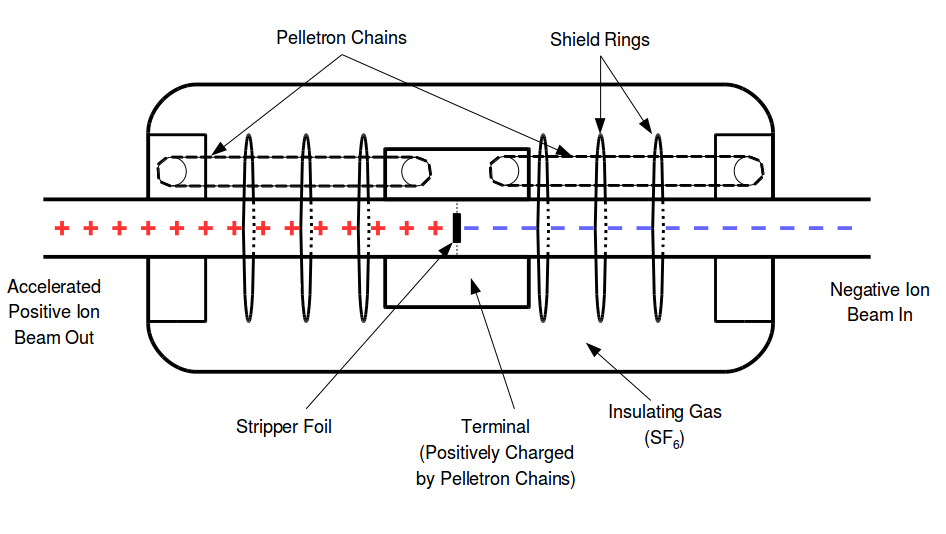
\includegraphics[scale=0.5]{tandem}
\end{center}
			\caption[Schematic of a MP tandem Van de Graaff accelerator]{Schematic of the MP Tandem Van de Graaff generator used at MLL. }
		\label{tandemDiagram}
\end{figure}
\FloatBarrier

\subsection{Beam Delivery}

After acceleration, the beam was then passed through a \SI{90}{\degree} analysing magnet, part of a beam energy calibration system\cite{dollingerfaestermann}. Combining the analysing magnet with analysing slits positioned after the magnets provided a feedback loop, where if the energy was too high or too low, this would be detected and the terminal voltage adjusted accordingly. This system was accurate to one part in $10^4$.

The beam was delivered to the target chamber by a series of quadrupole and dipole magnets to focus and steer respectively.

 ----------------------------------
%	SUBSECTION 2
%-----------------------------------
\subsection{Targets}
The tin targets used in these measurements were oxides, whereas cadmium targets were metallic. The targets were all prepared by evaporating the target material onto a carbon backing with a thickness of 10-\SI{30}{\micro\gram\per\centi\metre\squared}. Each target had a thickness of the order of \SI{100}{\micro\gram\per\centi\metre\squared}. These were mounted on a target ladder, which could hold up to four targets. There were also two more slots on the ladder. One of these was a collimator used for beam tuning, and one was left blank. The target ladders are shown in Figure~\ref{targetLadder}, with targets mounted. Each target could be moved into the path of the beam.

\begin{figure}[h]	
\hspace*{-0.5cm}
\begin{center}	
	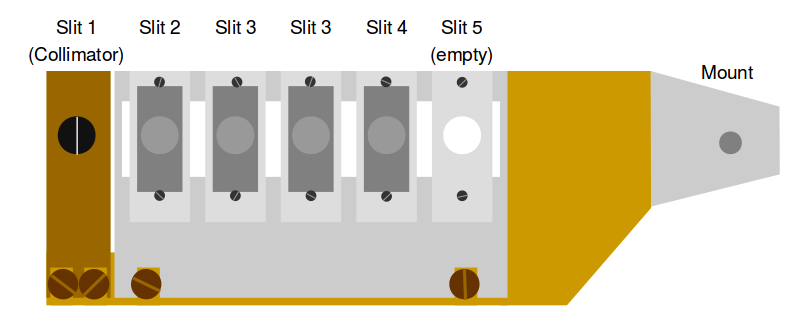
\includegraphics[scale=0.5]{targetladder}
\end{center}
			\caption[Diagram of the MLL target ladder]{Diagram of the target ladder. Slit 5 was empty because the mounting system physically prevented this slot from being moved into the correct position.}
		\label{targetLadder}
\end{figure}
\FloatBarrier

The target ladder was situated in a cylindrical target chamber. The chamber could be isolated from the beamline so it could be vented separately. This allowed the target ladder to be changed. Behind the target, a Faraday cup was positioned. This was connected to a Brookhaven current integrator\cite{bic} to measure the charge collected during each measurement. The spectrograph could be rotated around the target chamber to measure reaction products at different scattering angles. A cartoon of the target chamber is shown in Figure~\ref{targetChamber}, showing the positions of the spectrograph, target ladder, and beam line. At its entrance, there were adjustable slits for the horizontal and vertical collimation. The aperture size was set to \SI{14.03}{\milli\steradian}, except for at forward scattering angles, where it was set to \SI{7.25}{\milli\steradian}. This was done to prevent detector saturation due to large elastic scattering cross sections at these angles.

\begin{figure}[h]	
\hspace*{-0.5cm}
\begin{center}	
	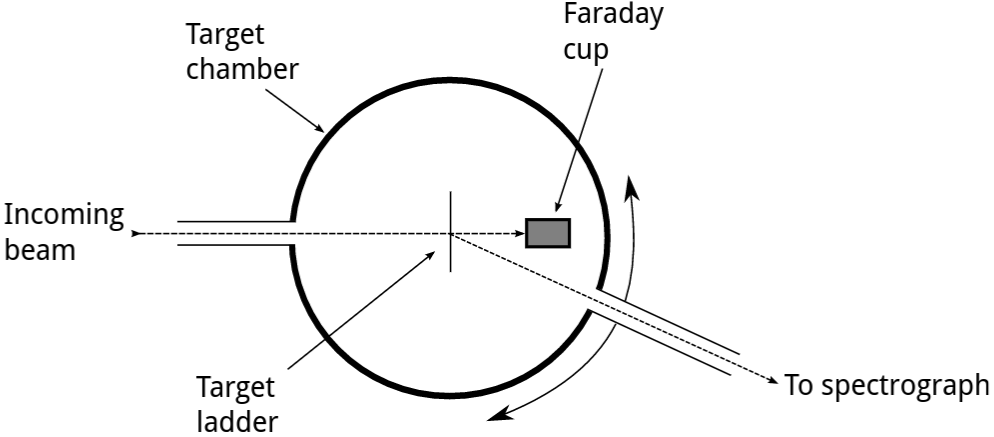
\includegraphics[scale=0.3]{targetchamber}
\end{center}
			\caption[Schematic of the Q3D target chamber]{A cartoon of the target chamber\cite{stuart}. Note that a faraday cup is placed behind the target to measure the beam current, and that the angle of the spectrograph can be altered.}
		\label{targetChamber}
\end{figure}
\FloatBarrier

 ----------------------------------
%	SUBSECTION 3
%-----------------------------------

\subsection{The Q3D Spectrograph}

The Q3D spectrograph separated ejectiles dispersively by their momentum. The position was measured to determine the momentum and excitation. A magnetic field was used to separate the ejectiles by applying a radial field.

Comparing the condition for circular motion

\begin{equation}
	F = \frac{mv^2}{\rho}\mathrm{,}
\end{equation}

where $F$ is the radial force experienced by the reaction product, $m$ is the mass of the reaction product, $v$ is the velocity, and $\rho$ is the radius of curvature, with the Lorentz equation for a charged particle moving perpendicular to a magnetic field,

\begin{equation}
	F = qBv\mathrm{,}
\end{equation}

where $F$ is the magnitude of the force, $q$ is the charge, $B$ is the magnetic field strength and $v$ is the velocity, gives 

\begin{equation}
	mv = qB\rho\mathrm{.}
\end{equation}

It can be seen that that the radius of curvature depends linearly on the momentum. This shows how the Q3D spectrometer separated ejectiles radially in the experiment.

The spectrograph did this with one quadrupole magnet and three dipole magnets. Figure~\ref{Q3D} is a cartoon of the spectrograph, showing the configuration of the magnets. It can be seen that the dipole magnets provided the radial bending.
 
\begin{figure}[h]	
\hspace*{-0.5cm}
\begin{center}	
	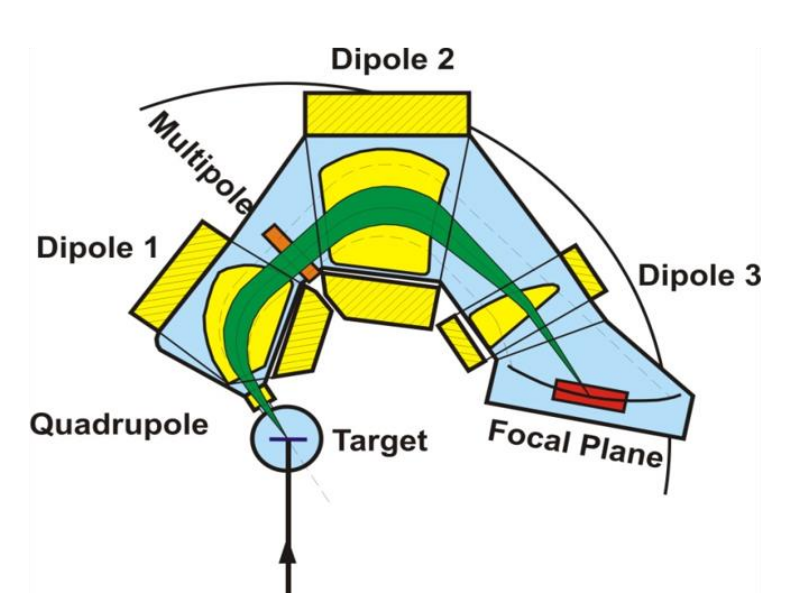
\includegraphics[scale=0.4]{benq3d}
\end{center}
			\caption[Schematic diagram of the Q3D magnetic spectrograph]{Sketch of the Q3D spectrograph, showing paths of ejectiles from the target to the focal plane.~\cite{dollingerfaestermann}}
		\label{Q3D}
\end{figure}
\FloatBarrier

While the dipole magnets provided the radial bending, the quadrupole increased the vertical acceptance of the spectrometer by focusing ejectiles into the focal plane of the detector. There was also a multipole element to correct for kinematic broadening~\cite{scheerer}. Overall, the ejectiles were vertically focused and bent horizontally into this focal plane, where a detector was placed.

 ----------------------------------
%	SUBSECTION 4
%-----------------------------------
\subsection{Focal Plane Detectors}

A detector system was placed along the focal plane to measure the position of the ejectiles, and therefore their momentum. Furthermore, the species of interest could be identified via the amount of energy lost in different parts of the detector system. 

There were three separate detectors in the focal plane detector system. Two were Multi-Wire Proportional Counters (MWPCs) and one was a plastic scintillator. The layout of the detectors is shown in Figure~\ref{detectorSketch}, with the MWPCs shown in front of the scintillator.

\begin{figure}[h]	
\hspace*{-0.5cm}
\begin{center}	
	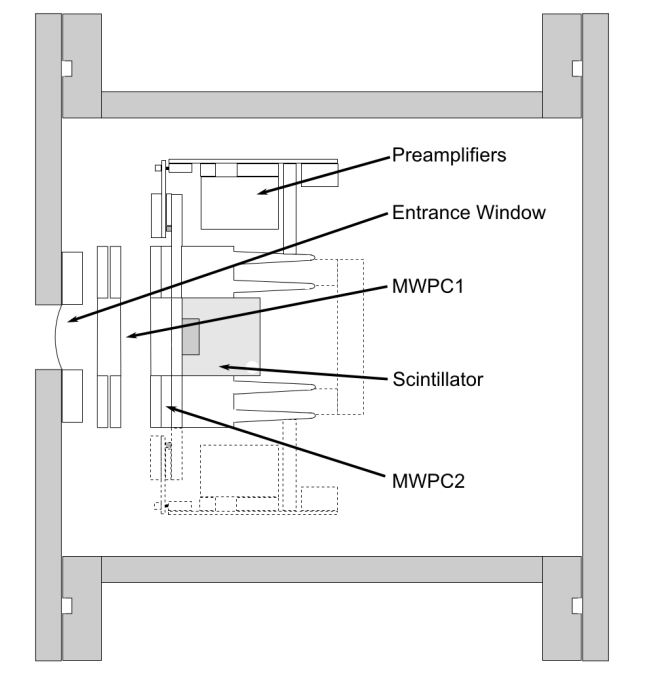
\includegraphics[scale=0.5]{focalplanesketch}
\end{center}
			\caption[Diagram of the focal plane detector]{Diagram of the layout of the focal plane detector~\cite{gillespie,mllreport}. The reaction products enter from the left, then pass through the two MWPCs and come to rest in the scintillator.}
		\label{detectorSketch}
\end{figure}
\FloatBarrier

An MWPC comprises a sandwich-like setup of parallel wires surrounded by isobutane gas, between two cathode foils. Upon being struck by a particle, the gas ionises. In regions of higher field near to the anode, this creates an avalanche. The electrons gather on an anode wire, while the ions gather on the cathode. The total signal from the anodes is proportional to the energy deposited by the incoming particle.

On the second of the MWPCs at the Munich Q3D, the cathode foil was split into multiple strips, where the charge accumulated on each could be measured. This allowed the position of the ionisation of the gas along the focal plane to be measured, and with it the position of the impact of the reaction product.

An event consisted of 3-6 adjacent strips registering a signal. The position was determined by fitting the collected charge on these strips with a Gaussian function. This process of determining the position is illustrated in Figure~\ref{posCathode}. Note that the cathode strips were equally spaced along the focal plane.

\begin{figure}[h]	
\hspace*{-0.5cm}
\begin{center}	
	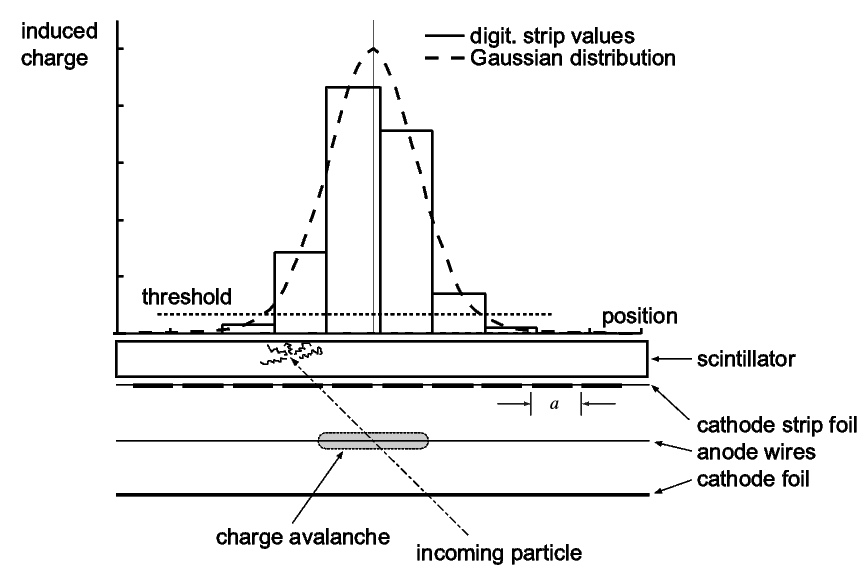
\includegraphics[scale=0.4]{cathodestrip}
\end{center}
			\caption[Illustration of the priciple of cathode strip detectors]{Illustration of the principle of the cathode strip method of focal plane position determination~\cite{mllreport}. $a$ is the repetition distance between cathode strips. A Gaussian distribution was fit to all of the cathode signals which exceed the threshold. }
		\label{posCathode}
\end{figure}
\FloatBarrier

Behind the two MWPCs, a plastic scintillator was placed to absorb the rest of the energy of an incoming reaction product. A scintillation detector works by converting the energy of an incoming particle into light, where the number of photons is proportional to the energy deposited by the particle. This light strikes a photocathode, which emits electrons via the photoelectric effect. The electrons are then multiplied in a photomultiplier tube, so the current is proportional to the energy deposited by the original incoming particle. This is then passed through a resistor, so the voltage across the resistor is then proportional to the energy of the initial reaction product.

The change in energy $\Delta E$ through both MWPCs was proportional to the anode signals. The corresponding final energy $E$ could be measured by the scintillator. Particles from the the reactions of interest could be identified through a comparison of the signals from the MWPCs and the scintillator.


\section{Experimental Considerations}

\subsection{Momentum Matching}

For \textsuperscript{116}Cd, \textsuperscript{114}Cd, and \textsuperscript{116}Sn, the states populated were in between the $N = 50, 82$ shell closures. This region corresponds to the $3s, 2d, 1h_{11/2}, \mathrm{and }1g_{7/2}$ orbitals. Some population of the states above and below may also be expected.

The (p,d) and (d,p) reactions favour population of states with low angular momentum.

The Q value of a reaction is the difference in rest mass energies of the initial and final states\cite{krane}. The deuteron is weakly bound, so the $Q$ value for these reactions are low. In contrast, the alpha particle is very strongly bound\cite{krane}, so transfer reactions involving alpha particles have high $Q$ values.

For a two body reaction with a moving projectile, and both target and recoil nuclei being stationary,

\begin{equation}
Q =\frac{p_i^2}{2m_i} - \frac{p_f^2}{2m_f}\mathrm{,}
\end{equation}

where $p_i$ and $m_i$ are the linear momentum and mass of the projectile, and $p_f$ and $m_f$ are the linear momentum and mass of the ejectile. The magnitude of the momentum transfer is 

\begin{equation}
q = |{\bf p}_i - {\bf p}_f|\mathrm{,}
\end{equation}

which depends on $Q$.

This linear momentum transfer affects the angular momentum transfer. Consider the classical expression for angular momentum

\begin{equation}
{\bf L} = {\bf r} \times {\bf p}\mathrm{,}
\end{equation}

where linear momentum is ${\bf p}$, and position relative to the centre of rotation is ${\bf r}$. In a direct reaction, ${\bf r}$ is approximately ${\bf R}$, the nuclear radius. Multiple step reactions are more likely if the projectile passes through the centre of the nucleus. Further away from the nucleus than the nuclear radius, any reaction becomes unlikely.

In this semiclassical approach, the angular momentum transfer increases with higher linear momentum transfer, and this increases with $Q$. For the reactions of interest, which have low $Q$ values, the population of states of low angular momentum was favoured.

\subsection{Angle and Energy Selection}


This semiclassical picture can also help with understanding how the angular distribution is affected by the angular momentum transfer $\delta {\bf l}$ and the beam energy $E_{\mathrm{lab}}$. The angular momentum transfer is

\begin{equation}
\Delta {\boldsymbol \ell} = {\bf R} \times {\bf q}\mathrm{,}
\end{equation}

so the maximum amount of transferred angular momentum is

\begin{equation}
\Delta \ell = R q \mathrm{.}
\end{equation}

Also,

\begin{equation} \label{momentumTransfer}
q = \sqrt{p_i^2 + p_f^2 - 2 p_i p_f \cos \theta}\mathrm{,}
\end{equation}

where $\theta$ is the scattering angle. With the knowledge that $R$ is constant, and that $p_i^2$ and $p_f^2$ are small due to the low $Q$ value of this reaction, it can be seen that $\delta l$ can be increased by increasing the scattering angle.

Conversely, the scattering angle can be reduced by increasing $E_{lab}$. For a given $q$, if the lab energy (and therefore projectile momentum) increases, the scattering angle becomes smaller. This is because the cross term in Equation~\ref{momentumTransfer} becomes large with a smaller scattering angle if $p_i$ and $p_f$ are larger. This means that angular distributions for all of the possible populated states become forward peaked at high energies.

This angle and energy dependence of $\delta l$ persist in a more rigorous DWBA model of the reaction, as shown in Figure~\ref{energyDists}. It is clear that a larger $\delta l$ results in a peak in cross-section at larger angles, increasing $E_{lab}$ makes the angular distributions more forward peaked, and that in general, low $\delta l$ is favoured. It is also shown that the cross sections for transfer reactions become much lower at smaller energies. This is because the projectiles are less likely to overcome the Coulomb barrier at lower energies.

\begin{figure}[h]	
\hspace*{-0.5cm}
\begin{center}
	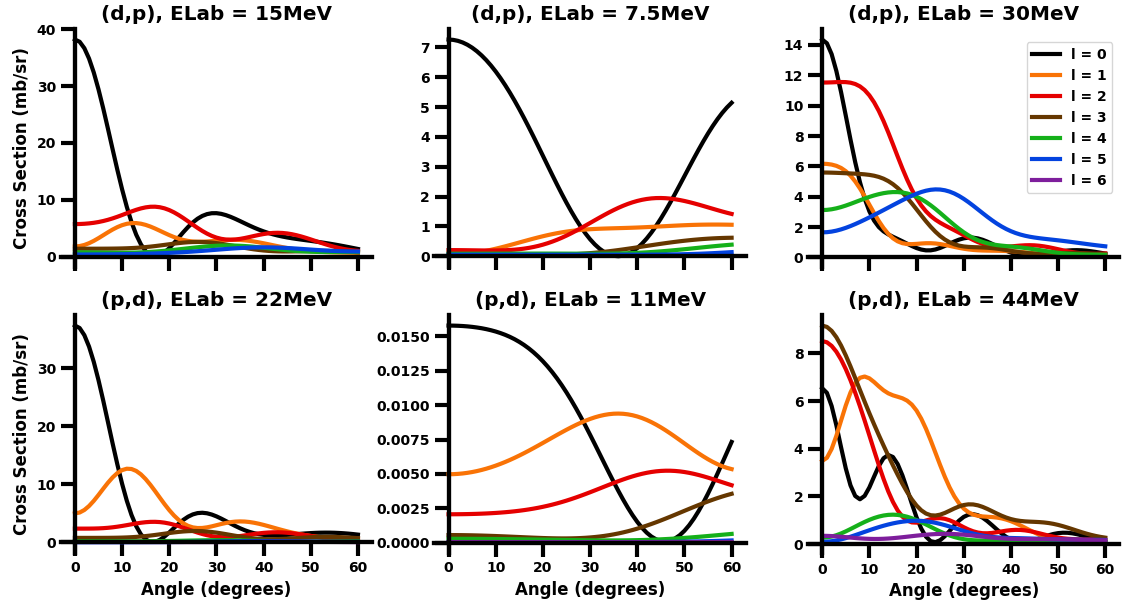
\includegraphics[width=\textwidth]{energydist}
\end{center}
			\caption[Angular distributions for (p,d) and (d,p) at different lab energies]{Angular distributions for (p,d) and (d,p) reactions on \textsuperscript{116}Cd. These are to a hypothetical ground state in the daughter nucleus.}
		\label{energyDists}
\end{figure}
\FloatBarrier

These effects were considered when selecting the angles and energies to measure at. \SI{22}{\mega\electronvolt} was chosen for all (p,d) reactions and \SI{15}{\mega\electronvolt} was chosen for (d,p). This was such that the peaks of different angular momentum states were distinct, and the cross-sections were sufficiently high. The angles where the $\ell = 0,2,4,5$ distributions peaked were chosen for the measuring angles. These were $\theta = (10, 18, 31, 40)^\mathrm{o}$ for (d,p), and $\theta = (8, 17, 31, 39)^\mathrm{o}$ for (p,d) An additional angle which lay at the peak of the $l = 3$ distribution ($\theta = 25^\mathrm{o}$ for (d,p), $\theta = 26^\mathrm{o}$ for (p,d)) was also measured with a smaller amount of beam time to distinguish between $\ell = 1$ and $\ell = 3$ states. The additional angle also ameliorated the obscuring effect of contaminants.

\subsection{Target Thickness} \label{ssec:tthick}

The thickness of the targets were an important consideration, because to calculate a cross-section, the number of particles that the beam may interact with must be known.

The target thickness was calculated by performing a reaction with a known cross-section, and deducing the target thickness from the yield collected for this reaction. The reaction used was elastic scattering, with the Rutherford cross-section used to calculate the cross-sections.

Rutherford scattering is the scattering of charged particles by the Coulomb field. The differential cross-section for Rutherford scattering in \si{\milli\barn\per\steradian}   is given by
\begin{equation}
\frac{\mathrm{d}\sigma}{\mathrm{d}\Omega}= 1.296\bigg(\frac{Z_bZ_t}{E_{\mathrm{lab}}}\bigg)^2\frac{1}{\sin^4\frac{\theta}{2}}
\end{equation}

where $Z_b$ and $Z_t$ are the proton numbers of the beam and target respectively, $E_{\mathrm{lab}}$ is the beam energy, and $\theta$ is the scattering angle\cite{rutherford,rutherfordformula}.

A beam energy and angle were selected such that the Rutherford cross-section was a valid approximation of the actual cross-section. This was best done at low energies so that the projectiles were less likely to get too close to the nucleus to assume pure Coulomb scattering. The chosen scattering angle could not be small because of the large scattering cross-section at these angles, which would swamp the detector. For \SI{9}{\mega\electronvolt} deuterons at a \SI{20}{\degree} scattering angle, which was the configuration used for target thickness measurements, it can be seen in Fig~\ref{elasticsRatio} that the elastic scattering cross section differed by 2\% from the Rutherford cross section.

\begin{figure}[h]	
\hspace*{-0.5cm}
\begin{center}
	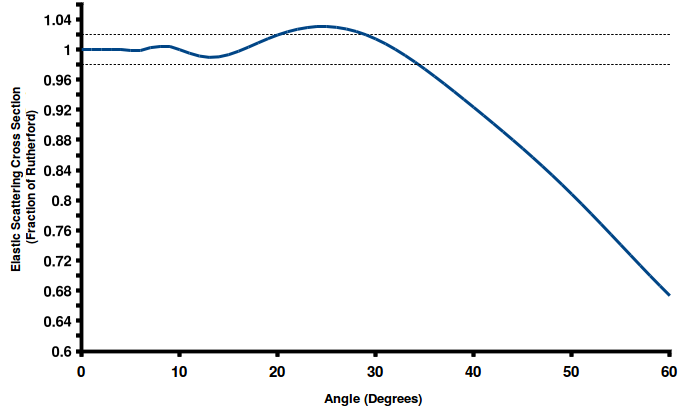
\includegraphics[width=\textwidth]{elasticsratio}
\end{center}
			\caption[Fraction of Rutherford cross-section for 9 MeV deuteron elastic scattering]{Fraction of Rutherford cross-section for 9 MeV deuteron elastic scattering. The dotted lines mark where the deviation from the Rutherford cross-section is 2\%. At 20 degrees, the deviation is approximately 2\%.}
		\label{elasticsRatio}
\end{figure}
\FloatBarrier


\subsection{Contaminants}

The targets were carbon-backed and some targets were oxides. Targets can also become oxidised with exposure to air. The targets also had varying isotopic purity.

The effect of light mass contaminants is the presence of large, broad peaks in the spectra. They are large because the states populated from reactions on \textsuperscript{16}O and \textsuperscript{12}C had large cross-sections from the reaction. The peaks were broad because they were out of focus, as the field was set to focus the ejectiles for reactions on the targets of interests which had a smaller kinematic shift. An example of a light-mass contaminant peak is shown in Fig~\ref{lmContaminant}.

\begin{figure}[h]	
\hspace*{-0.5cm}
\begin{center}
	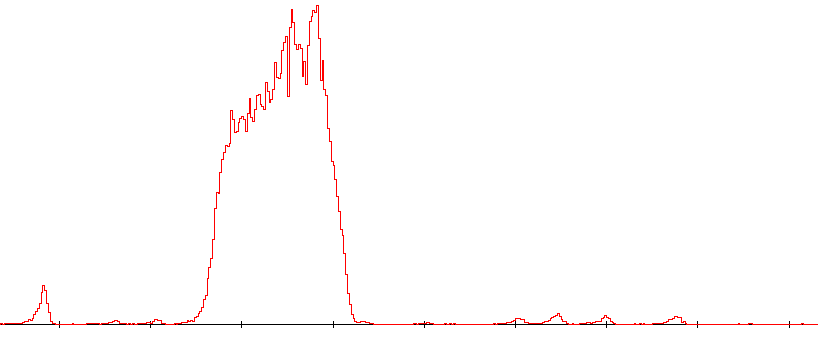
\includegraphics[width=\textwidth]{lmContaminant}
\end{center}
			\caption[Example of a light mass contaminant peak]{Example of a light mass contaminant peak. This is in the \textsuperscript{116}Sn (d,p) spectrum at a \SI{30}{\degree} scattering angle. The contaminant peak obscures states at approximately \SI{2.5}{\mega\electronvolt}. This is the \textsuperscript{12}C(d,p)\textsuperscript{13}C reaction, where the \textsuperscript{13}C is in its ground state.}
		\label{lmContaminant}
\end{figure}
\FloatBarrier

These light-mass contaminant peaks moved along the focal plane at different angle measurements. This meant that no state was obscured by the contaminant at every angle, but conversely it meant that more states were affected overall. The obscuring effect of the contaminant peaks was ameliorated by taking the bonus additional measurement.

As well as light mass contaminants, isotopic contaminants were present in the targets, because the enriching process did not fully erase the presence of other natural isotopes. Because each significant isotopic contaminant is at approximately 1\% enrichment, strong isotopic contaminant peaks appear with approximately 1\% of the yield of strong peaks for the desired reaction. This means they were visible, but at the limit of what could be seen, with less than 100 counts in the peaks. They were identifiable by a $qB\rho$ calibration of the spectra.

\subsection{Magnetic Field Settings}

The nuclear states were probed up to approximately \SI{4}{\mega\electronvolt}. This was not possible with one magnetic field setting of the Q3D, because the Q3D spectrometer had a large dispersion. This meant that states of different energy were separated more along the focal plane, and in this case so much that the 0-\SI{4}{\mega\electronvolt} range was not covered by the focal plane detector. In fact, the energy range covered by one measurement was approximately \SI{1}{MeV}.

This meant that multiple magnetic field settings had to be made. For (d,p), three field settings were used for each target at each angle, while for (p,d), four were used. It was ensured that there was an overlap of states between these measurements to allow for an accurate energy calibration. 
%% Chapter Template


\externaldocument{Chapter4}

\chapter{Analysis Methods} % Main chapter title

\label{Chapter5} % Change X to a consecutive number; for referencing this chapter elsewhere, use \ref{ChapterX}

\lhead{Chapter 5 \emph{Preliminary analysis}} % Change X to a consecutive number; this is for the header on each page - perhaps a shortened title



%----------------------------------------------------------------------------------------
%	SECTION 1
%----------------------------------------------------------------------------------------

\section{Data Sorting and Spectrum Extraction}

The first step in the analysis was to extract .spe format spectrum files from the ROOT\cite{root} files which contained the raw data. ROOT is a data analysis package often used with accelerator data. The ROOT data was sorted into a TTree, with data sorted into "leaves", each containing the signals from the MWPC anodes, the scintillators, and the position histogram.

The use of the  scintillator and anode signals was to select the desired reaction. Two of these signals were plotted against each other. The reaction products formed clusters, which could then be selected by a graphical cut. The selection of protons for \textsuperscript{116}Sn(d,p)\textsuperscript{117}Sn is shown in Figure~\ref{rootCut}.

\begin{figure}[h]	
\hspace*{-0.5cm}
\begin{center}	
	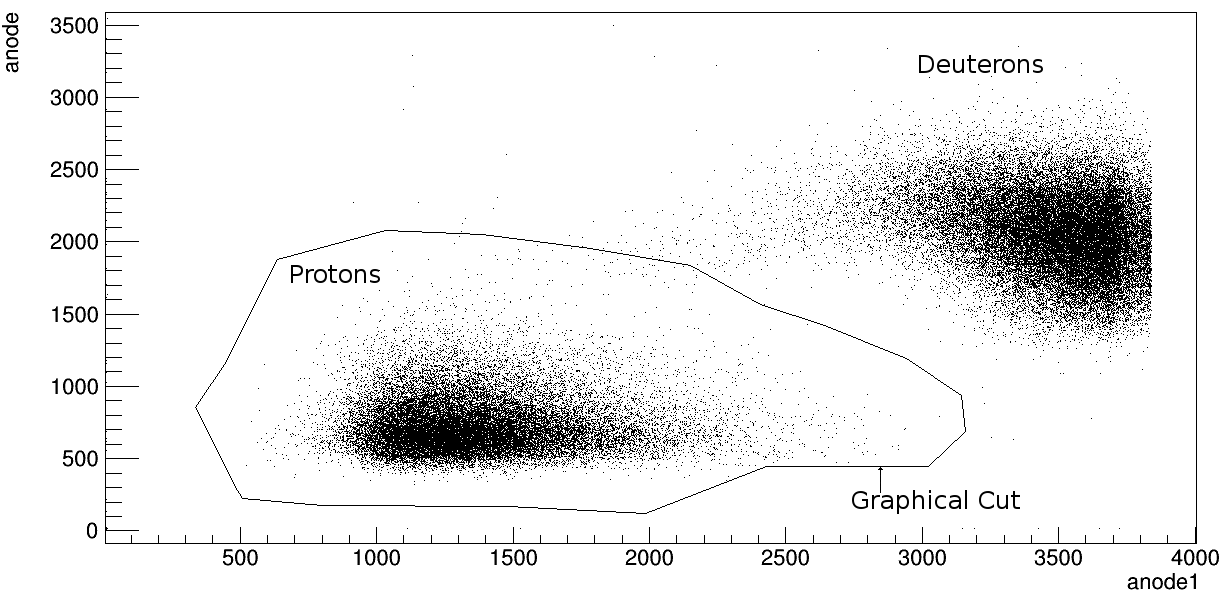
\includegraphics[scale=0.3]{rootcut}
\end{center}
			\caption[Using ROOT cuts for reaction selection]{The two MWPC anode signals plotted against each other for a deuteron beam on a \textsuperscript{116}Sn target. The signals from scattered deuterons and protons are in clusters, so can be separated by a graphical cut. }
		\label{rootCut}
\end{figure}
\FloatBarrier


Once each graphical cut was applied, the position histogram containing all of the counts in the cut was saved to a .spe spectrum format.

\section{Cross-Section Extraction}

The formula for determining the differential cross-section of a reaction from a yield $Y$ is

\begin{equation} \label{eq:yieldxsection}
\frac{\mathrm{d}\sigma}{\mathrm{d}\Omega} = \frac{Y}{\#t\#b\Delta\Omega\varepsilon},
\end{equation}

where $\#t$ is the number of target nuclei per unit area, $\#b$ is the integrated number of beam nuclei, $\Delta\Omega$ is the acceptance solid angle of the spectrograph, and $\varepsilon$ is a dead time correction to the beam current.

To calculate the cross-section for each reaction to each populated state, the corresponding yields were extracted from the spectra, and the other parameters also calculated. $\#b$ was measured by a Brookhaven Instruments Corporation beam current integrator (BIC)\cite{bic}. $\varepsilon$ was calculated by counting the fraction of events in the zero channel of the spectrum.

\subsection{Yield Extraction}

The yields for each state were extracted from the position spectrum by fitting each peak in the spectrum, and finding the area under the fitted curve by integrating it. The ansatz for the fitting was a skewed Gaussian function. The form of a skewed Gaussian function is the sum of a large Gaussian function and a smaller, offset Gaussian function to model the tails seen in the peaks. The fitting was done using the gf3 software from the Radware software package\cite{radware}. An example of a fit is shown in Figure~\ref{gf3Fit}.

\begin{figure}[h]	
\hspace*{-0.5cm}
\begin{center}	
	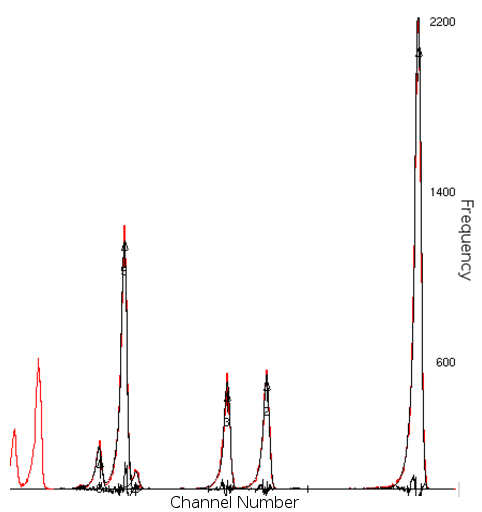
\includegraphics[scale=0.7]{gf3fit}
\end{center}
			\caption[Example fit curve of a spectrum]{An example of a set of peaks which have been fitted with skewed Gaussian fuunctions. This is for \textsuperscript{116}Cd(p,d)\textsuperscript{115}Cd, and the rightmost state is the \textsuperscript{115}Cd ground state. The peaks go from right to left in excitation energy. The red line is the spectrum histogram and the red line is the fitted line. The residuals are also shown. }
		\label{gf3Fit}
\end{figure}
\FloatBarrier

\subsection{Target Thickness}

The $\Delta\Omega$ and $\#t$ terms in Equation~\ref{eq:yieldxsection} were calculated together by using the elastic scattering measurements with the known Rutherford cross-section as discussed in Chapter 4. Because neither term changed between measurements for a specific target, they were substituted back into Equation~\ref{eq:yieldxsection} directly. However, a nominal aperture of \SI{14}{\milli\steradian} was used to approximate the target thickness. This nominal target thickness was then compared to the specification to check for defective foils.

\section{Energy Calibration}

The position of a peak along the spectrograph was proportional to the average momentum of the reaction products which composed the peak. The kinetic energy of these reaction products was proportional to the square of the momentum. There was a negative linear relationship between the kinetic energy of the reaction products and the excitation energy in the residual nucleus.

Overall, there was a negative quadratic relationship between the position of a peak along the focal plane and the excitation energy. Because of this, the ground state of the residual nucleus was always the rightmost peak. From here, the first few strong excited states were identified. The positions of these states were plotted against the energy, and a quadratic fit was made to the data.

Known, strong excited states of higher energy were identified by extrapolating this quadratic fit. This was done recursively, because the errors became very large quickly for the extrapolation, so identification became unreliable away from the known states. The energies of weaker states, unknown states, and previously unresolved doublets were calculated by interpoating the final fit. A calibration for the lowest lying states in \textsuperscript{117}Cd is shown in Figure~\ref{energyCalibration}.


\begin{figure}[h]	
\hspace*{-0.5cm}
\begin{center}	
	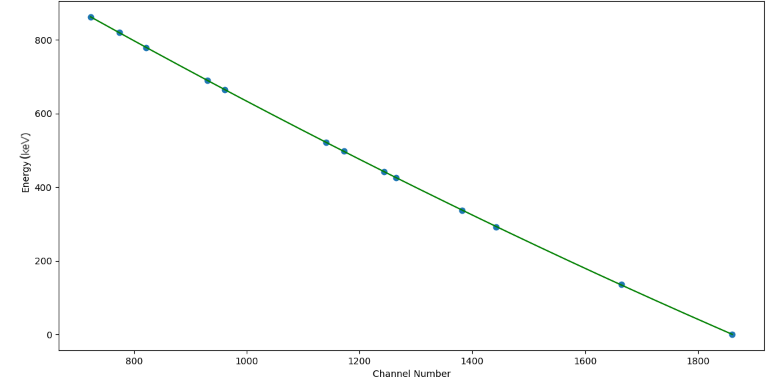
\includegraphics[width=\textwidth]{energycalibration}
\end{center}
			\caption[Energy calibration of the position spectrum]{The energy calibration for the measurement of the lowest MeV of states in \textsuperscript{117}Cd, from \textsuperscript{116}Cd(d,p)\textsuperscript{117}Cd measured at 18 degrees. A full error analysis has not been completed yet, but without errors this method still suffices for the identification of known states. The energies from the fit differ by approximately \SI{1}{\kilo\electronvolt} from previous data for strong states, which sets an approximate uncertainty on any energies calculated by this.}
		\label{energyCalibration}
\end{figure}
\FloatBarrier

The focal plane does not cover all of the energy region of interest, so several measurements were taken with an energy overlap, as discussed in Chapter 4. The overlap allowed the lowest lying states for measurements at higher energies to be identified.

\section{Angular Distributions and $\ell$  Assignment}

To find the occupancies for a given shell, the spectroscopic factors of all states of a given $j$ must be summed. The $\ell$  of each state must therefore be identified. This was done by measuring the angular distribution of the state. The angular distributions are distinct for different $\ell$, with peaks in the differential cross-section at different angles, as discussed in Chapter~\ref{Chapter4}.

The angular distributions for each value of $\ell$ were calculated. This was done by DWBA calculations using the PTOLEMY software\cite{ptolemy}. These distributions were compared to the experimental angular distributions. The experimental distribution was the same fraction smaller for each angle, so the entire calculated distribution was normalised by a constant value $N$, selected to minimize the $\chi^2$. The expression for $N$ for $n$ angle measurements was 

\begin{equation}
N = \frac{ 2 \sum_{i = 1}^{n} \sigma_i \, (\sigma_{i}^{\mathrm{DWBA}}) {}^2 \, s_i^{-2} } {\sum_{j = 1}^{n} \sigma_{j}^{\mathrm{DWBA}} s_j^{-2}}\mathrm{,}
\end{equation}

where $\sigma$ are the measured differential cross-sections, $\sigma^{\mathrm{DWBA}}$ are the cross-sections calculated by DWBA, and $s$ are the uncertainties on the measured cross-sections.

For each state, the normalised angular distributions for each $\ell$ were plotted on the same axes as the measured cross-sections. The $\chi^2$ was also displayed for each fitted distribution with a $\chi^2$ below double that of the fit with the lowest $\chi^2$. The angular momentum was then determined by comparing the value of the fit to the cross-section at the peak of the distribution, the $\chi^2$, and any previous $\ell$ assignment of the state. An example of an angular distribution comparison is shown in Figure~\ref{lAssignment}.

\begin{figure}[h]	
\hspace*{-0.5cm}
\begin{center}	
	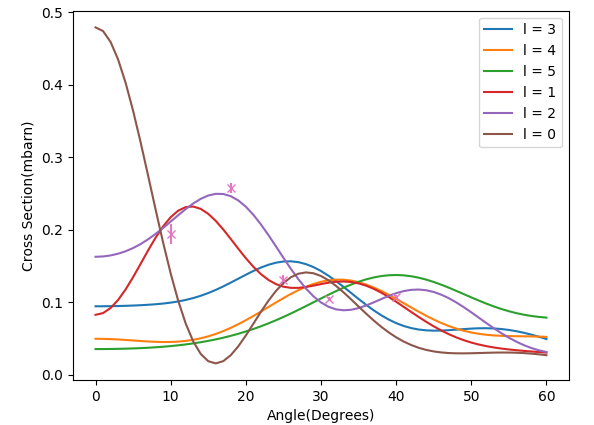
\includegraphics[scale = 0.75]{lassignment}
\end{center}
			\caption[Example of DWBA angular distributions normalised to a measured distribution ]{An example of an angular distribution compared to normalised DWBA distributions. This distribution is for \textsuperscript{116}Cd(d,p)\textsuperscript{117}Sn at a state of 522keV excitation energy. It was assigned as an $\ell = 2$ state.}
		\label{lAssignment}
\end{figure}
\FloatBarrier

\section{Spectroscopic Factors and Sum Rules}

The final section of the analysis will be to extract the spectroscopic factors from the distributions and to calculate the occupancies and vacancies using the Macfarlane and French sum rules. This has not been attempted yet. The cross-section at the peak of each distribution will be divided by the DWBA cross-section at that angle. This will be the spectroscopic factor for each state. Each state will be sorted by its $\ell$, and an occupancy or vacancy will be calculated for each orbital by summing all of the spectroscopic factors for that orbital. This will be normalized to account for missing strength at higher excitation energies. This will be done such that the normalized occupancies and vacancies will sum to $2j + 1$.

\section{Preliminary Assignments}

So far, a full energy calibration has only been done for \textsuperscript{116}Cd(d,p)\textsuperscript{117}Cd, for energies up to \SI{1.2}{\mega\electronvolt}. Angular distributions have been extracted for the states in this region. As well as this, the three states of lowest energy in \textsuperscript{116}Cd(p,d)\textsuperscript{117}Cd have also been measured.

The first three states of the (p,d) had angular distributions which closely resemble the theory. The $\ell = 5$ state was not as accurate because of the poor momentum matching for this reaction. These distributions are shown in Figure~\ref{pdDistributions}.


\begin{figure}[h]	
\hspace*{-0.5cm}
\begin{center}	
	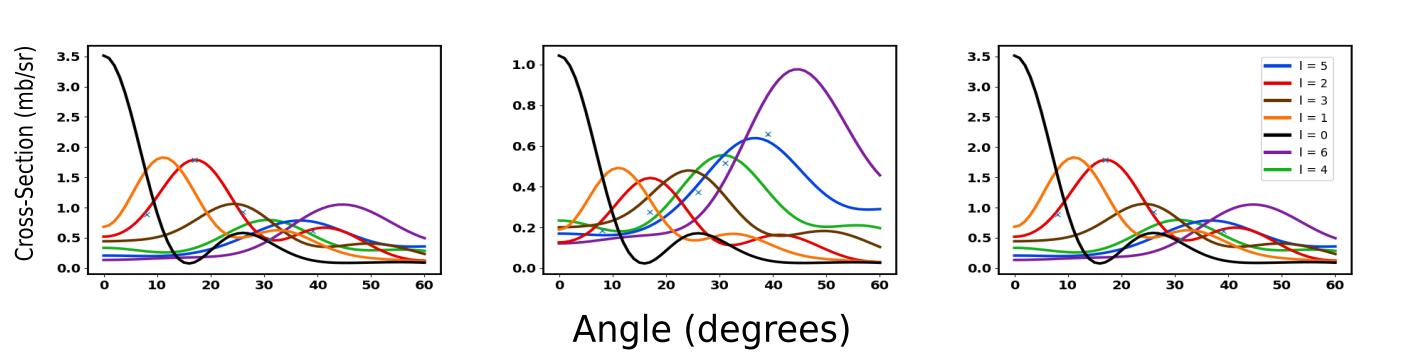
\includegraphics[width  = \textwidth]{pd}
\end{center}
			\caption[\textsuperscript{116}Cd(p,d)\textsuperscript{115}Cd angular distributions for the strongest states ]{Angular distributions for the he first three states in \textsuperscript{115}Cd. These have $\ell = 0,5,2$ respectively.}
		\label{pdDistributions}
\end{figure}
\FloatBarrier

For the (d,p), the distributions did not fit as well, particularly for $\ell = 0$ states. They were still identifiable, but the poor fit means that the spectroscopic factors for these graphs will be unreliable. The $\ell = 2$
fit the distributons well, as in Figure~\ref{lAssignment}. All of the angular distributions for (d,p), with all of the  possible theoretical distributions for each $\ell$ , are shown in Figure~\ref{dpDistributions}.

\begin{figure}[h]	
\vspace*{-2cm}
    \makebox[\linewidth]{
        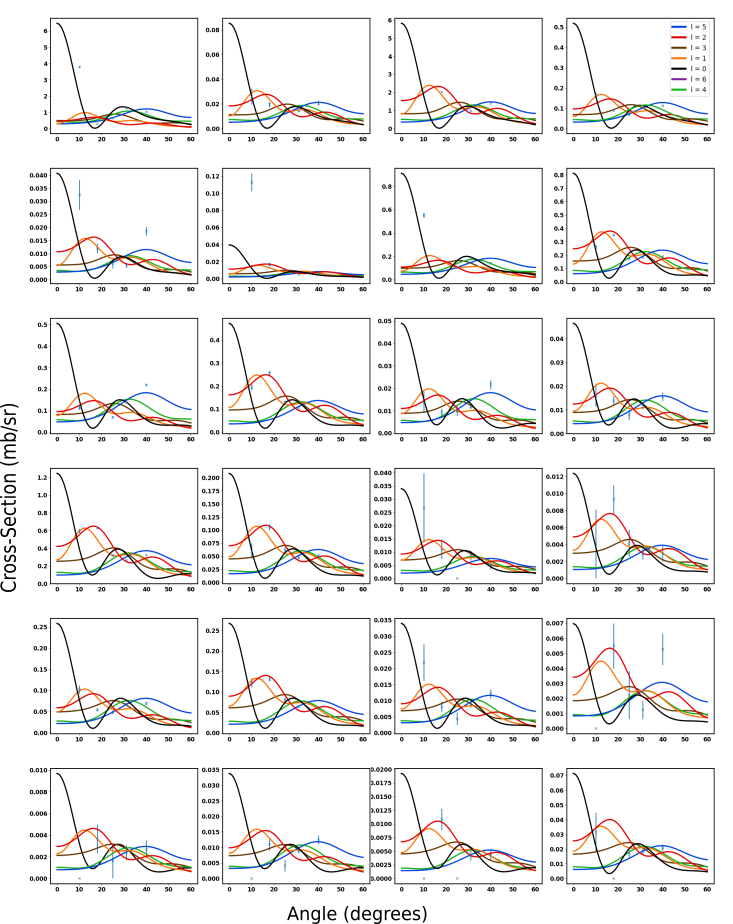
\includegraphics[width=1.3\linewidth]{dp}	
		}
			\caption[The angular distributions for (d,p) reactions to states in \textsuperscript{117}Cd]{The angular distributions for (d,p) to states in \textsuperscript{117}Cd. These are up to 1.2 MeV in excitation energy. For $\ell = 0$ states, The DWBA cross-sections do not match the experimental cross-sections very well.}
		\label{dpDistributions}
\end{figure}
\FloatBarrier


The cross-sections for the (d,p) on \textsuperscript{116}Sn did not match with previous measurements\cite{stuart}. Early results from another recent experiment to check these measurements were consistent with the earlier measurements rather than those discussed in this report. The entirety of the (d,p) data may have been incorrect. This will be verified if the normalisation for occupancies and vacancies for \textsuperscript{116}Cd match the tin. 
%% Chapter Template

\chapter{Conclusions} % Main chapter title

\label{Chapter6} % Change X to a consecutive number; for referencing this chapter elsewhere, use \ref{ChapterX}

\lhead{Chapter6. \emph{Conclusions}} % Change X to a consecutive number; this is for the header on each page - perhaps a shortened title

%----------------------------------------------------------------------------------------
%	SECTION 1
%----------------------------------------------------------------------------------------

\section{Summary}
(p,d) and (d,p) transfer reactions were done on \textsuperscript{116}Cd, \textsuperscript{114}Cd, and \textsuperscript{116}Sn. These were done using the Q3D magnetic spectrometer at the Maier-Leibnitz Laboratorium. These nuclei are interesting because \textsuperscript{116}Cd and \textsuperscript{116}Sn are the parent and daughter nuclei of a potential $0\nu2\beta$ reaction. The reactions were done to extract the occupancies of the valence orbitals, which helps when constructing models to determine the $0\nu2\beta$ matrix element. This allows the calculation of the neutrino mass upon the detection of the process.

The data from these reactions are currently being analysed. The yields have all been extracted. Angular distributions were extracted for the lowest-lying states in (p,d), and the angular distributions match what has already been measured. It just remains to do energy calibrations for the rest of the states, calculate spectroscopic factors from the peaks of the distributions, and sum them to find the occupancies. For the (d,p) reaction however, further review is required.
\newpage
%-----------------------------------
%	SUBSECTION 1
%-----------------------------------
\section{Outlook}

The spectroscopic factors and occupancies first need to be found for these targets. After this, (\textsuperscript{3}He, $\alpha$) data which was recently collected will be analysed, which better probes states of higher $\ell$ than proton or deuteron beams. As well as this, the (d,p) reaction has been repeated on the same targets for low excitation energies. This will be analysed to check that the cross-sections are consistent between that experiment and the experiment discussed in this report. All of these occupancies will also be compared to occupancies in the theoretical frameworks for the matrix elements for $0\nu2\beta$ decay to check that those frameworks reproduce the reality of the nuclear structure.

With the arrival of more experimental data comes the need for more sophisticated data analysis. Currently, the gf3 package from Radware is used to fit spectra. An automatic fitting program will be designed to replace it. This will need to be able to identify multiplet states and contaminants and extract yields for all states. Preliminary discussions suggest using machine learning to identify the nature of each peak will be beneficial.

 
%\input{Chapters/Chapter7} 

%----------------------------------------------------------------------------------------
%	THESIS CONTENT - APPENDICES
%----------------------------------------------------------------------------------------

\addtocontents{toc}{\vspace{2em}} % Add a gap in the Contents, for aesthetics

\appendix % Cue to tell LaTeX that the following 'chapters' are Appendices

% Include the appendices of the thesis as separate files from the Appendices folder
% Uncomment the lines as you write the Appendices

%% Appendix A

\chapter{Raw spectroscopic factors} % Main appendix title

\label{AppendixA} % For referencing this appendix elsewhere, use \ref{AppendixA}

\lhead{Appendix A.} % This is for the header on each page - perhaps a shortened title

Tabulated below are the cross sections, l assignments and the spectroscopic factors of the distributions for the $^{150}$Nd and $^{150}$Sm targets.

\begin{table}
\caption{Energies, cross sections, assigned $\ell$ values and spectroscopic factors for $^{150}$Nd}
\begin{tabular}{c c c c c c c}
\hline \hline
Energy (MeV) & $\sigma_{12}$ & $\sigma_{18}$ & $\sigma_{25}$ & $\sigma_{38}$ & Assigned $\ell$ & S\\
\hline \hline
0.000 (4) & 0.062 (8) & 0.097 (15) & 0.077 (10) & 0.044 (10) & 2 & 0.009 (1) \\
0.009 (5) & 0.036 (6) & 0.031 (9) & 0.042 (7) & 0.019 (5) & 3 & 0.004 (1) \\
0.109 (3) & 0.673 (27) & 0.852 (34) & 0.976 (36) & 0.493 (11) & 3 & 0.101 (4) \\
0.139 (3) & 0.200 (14) & 0.244 (19) & 0.288 (19) & 0.121 (5) & 3 & 0.030 (2) \\
0.165 (20) & 1.421 (39) & 0.920 (33) & 0.510 (26) & 0.359 (9) & 1 & 0.097 (3) \\
0.190 (6) & 0.061 (8) & 0.066 (9) & 0.077 (11) & 0.039 (3) & 3 & 0.008 (1) \\
0.220 (5) & 0.060 (8) & 0.081 (11) & 0.084 (10) & 0.154 (6) & 5 & 0.078 (3) \\
0.258 (7) & 0.293 (18) & 0.195 (16) & 0.136 (14) & 0.070 (4) & 1 & 0.078 (3) \\
0.271 (8) & 0.124 (12) & 0.210 (16) & 0.304 (21) & 0.236 (8) & 3 & 0.033 (2) \\
0.285 (7) & 0.510 (24) & 0.308 (23) & 0.161 (15) & 0.118 (6) & 1 & 0.035 (2) \\
0.315 (10) & 0.477 (61) & 0.446 (33) & 0.596 (104) & 0.211 (17) & 3 & 0.065 (11) \\
0.320 (11) & 0.303 (51) & 0.548 (36) & 0.507 (104) & 0.273 (15) & 3 & 0.056 (11) \\
0.332 (14) & 0.222 (22) & 0.181 (22) & 0.086 (15) & 0.086 (6) & 1 & 0.016 (2) \\
0.340 (17) & 0.051 (14) & 0.066 (17) & 0.062 (11) & 0.166 (7) & 5 & 0.126 (5) \\
0.365 (18) & 1.807 (44) & 1.012 (48) & 0.487 (26) & 0.452 (11) & 1 & 0.127 (3) \\
0.403 (17) & 0.485 (22) & 0.219 (18) & 0.103 (12) & 0.122 (6) & 1 & 0.034 (2) \\
0.442 (6) & 0.027 (6) & 0.033 (6) & 0.036 (9) & 0.018 (2) & 3 & 0.004 (1) \\
0.450 (3) & 0.212 (16) & 0.274 (18) & 0.296 (21) & 0.152 (6) & 3 & 0.034 (2) \\
0.460 (6) & 0.025 (6) & 0.038 (8) & 0.032 (9) & 0.026 (2) & 2 & 0.004 (1) \\
0.482 (3) & 0.233 (16) & 0.136 (12) & 0.288 (20) & 0.102 (5) & 0 & 0.041 (3) \\
0.512 (4) & 0.078 (9) & 0.083 (9) & 0.069 (10) & 0.085 (5) & 5 & 0.046 (2) \\
0.547 (13) & 1.999 (46) & 1.153 (36) & 0.537 (26) & 0.467 (11) & 1 & 0.145 (3) \\
0.570 (3) & 0.171 (14) & 0.207 (15) & 0.105 (12) & 0.078 (4) & 2 & 0.025 (2) \\
0.589 (5) & 0.140 (12) & 0.156 (14) & 0.125 (13) & 0.105 (5) & 2 & 0.019 (2) \\
0.615 (7) & 0.025 (6) & 0.032 (7) & 0.030 (7) & 0.025 (3) & 2,3 & 0.004 (1) \\
0.646 (20) & 0.349 (19) & 0.386 (21) & 0.360 (22) & 0.444 (11) & 5 & 0.251 (6) \\
0.708 (7) & 2.436 (51) & 3.209 (61) & 1.749 (48) & 1.114 (17) & 2 & 0.403 (8) \\
0.740 (9) & 1.182 (36) & 1.468 (41) & 0.808 (32) & 0.547 (12) & 2 & 0.187 (5) \\
0.797 (5) & 0.134 (15) & 0.149 (14) & 0.084 (12) & 0.059 (4) & 2 & 0.019 (2) \\
0.805 (5) & 0.115 (18) & 0.152 (16) & 0.182 (19) & 0.064 (8) & 3 & 0.023 (2) \\
0.814 (10) & 1.276 (38) & 0.989 (35) & 1.564 (49) & 0.655 (13) & 0 & 0.253 (7) \\
0.828 (5) & 0.074 (13) & 0.109 (20) & 0.070 (7) & 0.032 (6) & 2 & 0.014 (3) \\
0.837 (23) & 0.228 (17) & 0.150 (24) & 0.071 (21) & 0.103 (6) & 1 & 0.017 (1) \\
0.861 (9) & 0.029 (5) & 0.051 (11) & 0.047 (9) & 0.062 (3) & 5 & 0.037 (2) \\
0.880 (12) & 0.611 (26) & 0.802 (31) & 0.419 (24) & 0.294 (9) & 2 & 0.108 (4) \\
0.923 (5) & 0.063 (11) & 0.083 (10) & 0.059 (8) & 0.044 (4) & 2 & 0.011 (1) \\
0.954 (4) & 0.020 (5) & 0.029 (7) & 0.060 (9) & 0.037 (3) & 3,5 & 0.008 (1) \\
0.962 (3) & 0.130 (12) & 0.201 (15) & 0.090 (15) & 0.061 (4) & 2 & 0.028 (2) \\
0.984 (6) & 3.352 (60) & 1.731 (44) & 4.850 (82) & 1.531 (20) & 0 & 0.697 (12) \\
1.027 (4) & 0.352 (19) & 0.230 (16) & 0.093 (12) & 0.088 (5) & 1 & 0.028 (2) \\
1.045 (18) & 0.281 (18) & 0.412 (22) & 0.261 (19) & 0.132 (6) & 2 & 0.059 (3) \\
1.066 (8) & 0.033 (6) & 0.081 (11) & 0.059 (8) & 0.020 (2) & 2 & 0.012 (2) \\
1.082 (5) & 0.057 (7) & 0.040 (8) & 0.018 (5) & 0.017 (2) & 1 & 0.005 (1) \\
1.129 (14) & 0.454 (24) & 0.556 (29) & 0.395 (16) & 0.207 (8) & 2 & 0.083 (4) \\
\hline \hline
\end{tabular}
\label{Nd1}
\end{table}

\begin{table}
\caption{Energies, cross sections, assigned $\ell$ values and spectroscopic factors for $^{150}$Nd}
\begin{tabular}{c c c c c c c}
\hline \hline
Energy (MeV) & $\sigma_{12}$ & $\sigma_{18}$ & $\sigma_{25}$ & $\sigma_{38}$ & Assigned $\ell$ & S\\
\hline \hline
1.148 (3) & 0.102 (11) & 0.143 (15) & 0.091 (10) & 0.057 (5) & 2 & 0.021 (2) \\
1.177 (3) & 0.082 (9) & 0.059 (7) & 0.023 (5) & 0.019 (3) & 1 & 0.007 (1) \\
1.188 (4) & 0.075 (8) & 0.032 (11) & 0.028 (6) & 0.029 (3) & 1 & 0.006 (1) \\
1.218 (23) & 0.048 (8) & 0.035 (8) & 0.018 (5) & 0.021 (3) & 1 & 0.004 (1) \\
1.231 (3) & 0.054 (9) & 0.026 (8) & 0.103 (11) & 0.025 (2) & 0 & 0.017 (2) \\
1.244 (3) & 0.098 (10) & 0.119 (13) & 0.082 (10) & 0.053 (4) & 2 & 0.019 (2) \\
1.281 (23) & 0.165 (15) & 0.096 (12) & 0.065 (9) & 0.061 (4) & 1 & 0.014 (1) \\
1.359 (5) & 0.090 (9) & 0.093 (9) & 0.100 (12) & 0.035 (3) & 3 & 0.014 (2) \\
1.419 (4) & 0.025 (5) & 0.034 (6) & 0.012 (5) & 0.012 (2) & 2 & 0.006 (1) \\
1.468 (3) & 0.077 (9) & 0.057 (8) & 0.026 (6) & 0.019 (2) & 1 & 0.007 (1) \\
1.483 (4) & 0.074 (9) & 0.052 (7) & 0.048 (9) & 0.021 (2) & 1,2 & 0.007 (1) \\
1.497 (15) & 0.027 (5) & 0.039 (6) & 0.036 (7) & 0.014 (2) & 2 & 0.007 (1) \\
1.507 (22) & 0.507 (22) & 0.285 (17) & 0.127 (13) & 0.105 (5) & 1 & 0.045 (2) \\
1.535 (21) & 0.209 (14) & 0.119 (15) & 0.086 (11) & 0.047 (5) & 1 & 0.019 (1) \\
1.554 (4) & 0.238 (15) & 0.136 (13) & 0.087 (11) & 0.067 (4) & 1 & 0.021 (1) \\
1.565 (3) & 0.027 (5) & 0.033 (5) & 0.044 (8) & 0.013 (2) & 3 & 0.007 (1) \\
1.622 (3) & 0.148 (12) & 0.117 (7) & 0.104 (12) & 0.064 (4) & 1 & 0.013 (1) \\
1.628 (4) & 0.060 (8) & 0.042 (6) & 0.023 (5) & 0.036 (3) & 1 & 0.006 (1) \\
1.690 (3) & 0.059 (7) & 0.075 (8) & 0.065 (10) & 0.034 (3) & 2 & 0.014 (2) \\
1.705 (3) & 0.111 (10) & 0.143 (11) & 0.089 (11) & 0.086 (5) & 2 & 0.027 (2) \\
1.718 (4) & 0.075 (8) & 0.106 (11) & 0.073 (10) & 0.041 (3) & 2 & 0.020 (2) \\
1.732 (3) & 0.068 (8) & 0.089 (10) & 0.058 (9) & 0.032 (3) & 2 & 0.017 (2) \\
1.748 (4) & 0.111 (10) & 0.123 (12) & 0.069 (10) & 0.044 (3) & 2 & 0.024 (2) \\
1.778 (5) & 0.056 (7) & 0.032 (6) & 0.017 (5) & 0.015 (2) & 1 & 0.005 (1) \\
1.795 (8) & 0.359 (32) & 0.422 (32) & 0.272 (19) & 0.150 (6) & 2 & 0.084 (6) \\
1.799 (3) & 0.099 (16) & 0.077 (16) & 0.063 (9) & 0.035 (3) & 1,2 & 0.009 (2) \\
1.829 (17) & 0.058 (7) & 0.050 (7) & 0.085 (10) & 0.021 (2) & 0 & 0.018 (2) \\
1.867 (3) & 0.295 (25) & 0.406 (20) & 0.241 (18) & 0.128 (5) & 2 & 0.084 (4) \\
1.872 (3) & 0.055 (12) & 0.075 (8) & 0.049 (8) & 0.031 (3) & 2 & 0.015 (2) \\
1.890 (3) & 0.068 (8) & 0.075 (8) & 0.053 (8) & 0.034 (3) & 2 & 0.016 (2) \\
1.916 (3) & 0.039 (6) & 0.036 (6) & 0.023 (6) & 0.017 (2) & 1 & 0.004 (1) \\
1.966 (21) & 0.072 (8) & 0.059 (8) & 0.041 (9) & 0.034 (3) & 1 & 0.007 (1) \\
1.983 (17) & 0.095 (9) & 0.112 (12) & 0.065 (9) & 0.048 (4) & 2 & 0.024 (3) \\
1.990 (5) & 0.164 (15) & 0.175 (16) & 0.084 (10) & 0.059 (4) & 2 & 0.038 (3) \\
2.006 (16) & 0.018 (4) & 0.035 (6) & 0.021 (6) & 0.014 (2) & 2 & 0.008 (1) \\
2.033 (3) & 0.241 (15) & 0.231 (15) & 0.404 (23) & 0.087 (4) & 0 & 0.082 (5) \\
2.049 (4) & 0.038 (7) & 0.039 (6) & 0.051 (8) & 0.021 (2) & 3 & 0.009 (1) \\
2.065 (3) & 0.030 (6) & 0.060 (8) & 0.037 (7) & 0.022 (2) & 2 & 0.013 (2) \\
2.083 (12) & 0.147 (12) & 0.152 (15) & 0.093 (11) & 0.063 (4) & 2 & 0.035 (3) \\
2.087 (15) & 0.423 (22) & 0.438 (20) & 0.325 (21) & 0.169 (6) & 2 & 0.100 (5) \\
2.097 (18) & 0.068 (11) & 0.075 (9) & 0.067 (10) & 0.033 (2) & 2 & 0.017 (2) \\
2.101 (17) & 0.128 (11) & 0.086 (12) & 0.132 (14) & 0.036 (3) & 0 & 0.045 (4) \\
2.125 (4) & 0.103 (10) & 0.060 (10) & 0.052 (8) & 0.027 (2) & 1,2,3 & 0.009 (1) \\
2.186 (3) & 0.035 (6) & 0.076 (11) & 0.037 (7) & 0.017 (2) & 2 & 0.018 (3) \\
2.226 (3) & 0.149 (12) & 0.138 (12) & 0.147 (14) & 0.058 (3) & 3 & 0.026 (3) \\
\hline \hline
\end{tabular}
\label{Nd2}
\end{table}

\begin{table}
\caption{Energies, cross sections, assigned $\ell$ values and spectroscopic factors for $^{150}$Nd}
\begin{tabular}{c c c c c c c}
\hline \hline
Energy (MeV) & $\sigma_{12}$ & $\sigma_{18}$ & $\sigma_{25}$ & $\sigma_{38}$ & Assigned $\ell$ & S\\
\hline \hline
2.235 (4) & 0.050 (7) & 0.072 (9) & 0.028 (6) & 0.022 (2) & 2 & 0.027 (3) \\
2.253 (4) & 0.052 (7) & 0.069 (10) & 0.037 (6) & 0.026 (2) & 2 & 0.024 (3) \\
2.269 (3) & 0.027 (5) & 0.081 (11) & 0.044 (8) & 0.022 (2) & 2 & 0.020 (3) \\
2.276 (5) & 0.146 (12) & 0.109 (13) & 0.106 (12) & 0.063 (4) & 1,2,3 & 0.016 (1) \\
2.285 (5) & 0.146 (33) & 0.160 (13) & 0.092 (11) & 0.071 (4) & 2 & 0.040 (3) \\
2.291 (20) & 0.265 (28) & 0.341 (18) & 0.192 (15) & 0.121 (5) & 2 & 0.086 (5) \\
2.303 (3) & 0.211 (14) & 0.188 (14) & 0.175 (15) & 0.085 (4) & 1,2,3 & 0.051 (4) \\
2.320 (5) & 0.083 (9) & 0.077 (8) & 0.060 (9) & 0.025 (2) & 1,2,3 & 0.022 (2) \\
2.369 (1) & 0.039 (6) & 0.052 (7) & 0.050 (8) & 0.022 (2) & 2 & 0.013 (2) \\
2.389 (5) & 0.044 (7) & 0.038 (6) & 0.063 (10) & 0.024 (2) & 3 & 0.012 (2) \\
2.396 (5) & 0.080 (9) & 0.092 (10) & 0.074 (10) & 0.044 (3) & 2 & 0.024 (3) \\
2.412 (7) & 0.162 (14) & 0.145 (13) & 0.108 (13) & 0.075 (4) & 1 & 0.018 (2) \\
2.526 (5) & 0.048 (7) & 0.043 (7) & 0.044 (8) & 0.019 (2) & 2,3 & 0.009 (2) \\
2.544 (3) & 0.109 (11) & 0.090 (10) & 0.141 (14) & 0.056 (3) & 3 & 0.028 (3) \\
2.583 (3) & 0.050 (7) & 0.068 (9) & 0.048 (8) & 0.024 (2) & 2 & 0.020 (3) \\
2.604 (7) & 0.074 (9) & 0.072 (9) & 0.058 (9) & 0.032 (3) & 2 & 0.021 (3) \\
2.623 (9) & 0.129 (12) & 0.131 (12) & 0.135 (13) & 0.058 (5) & 3 & 0.027 (3) \\
\hline \hline
\end{tabular}
\label{Nd3}
\end{table}

\begin{table}
\caption{Energies, cross sections, assigned $\ell$ values and spectroscopic factors for $^{150}$Sm}
\begin{tabular}{c c c c c c c}
\hline \hline
Energy (MeV) & $\sigma_{12}$ & $\sigma_{18}$ & $\sigma_{25}$ & $\sigma_{38}$ & Assigned $\ell$ & S\\
\hline \hline
0.000 (20) & 1.779 (46) & 2.298 (43) & 2.824 (65) & 1.615 (27) & 2 & 0.294 (5) \\
0.022 (10) & 0.039 (10) & 0.096 (11) & 0.098 (20) & 0.046 (6) & 2 & 0.012 (1) \\
0.276 (3) & 0.235 (17) & 0.395 (20) & 0.267 (31) & 0.151 (9) & 2 & 0.056 (3) \\
0.285 (3) & 0.093 (12) & 0.092 (23) & 0.052 (19) & 0.162 (9) & 5 & 0.103 (6) \\
0.350 (11) & 2.417 (50) & 1.729 (40) & 1.046 (116) & 0.742 (18) & 1 & 0.203 (4) \\
0.397 (5) & 0.126 (13) & 0.089 (10) & 0.075 (18) & 0.043 (5) & 1 & 0.011 (1) \\
0.529 (11) & 1.549 (41) & 0.948 (27) & 0.396 (24) & 0.539 (16) & 1 & 0.135 (4) \\
0.558 (22) & 0.117 (11) & 0.184 (13) & 0.202 (17) & 0.097 (7) & 3 & 0.029 (2) \\
0.578 (4) & 0.085 (11) & 0.112 (12) & 0.063 (9) & 0.032 (5) & 2 & 0.018 (2) \\
0.587 (5) & 0.116 (12) & 0.078 (9) & 0.035 (7) & 0.045 (5) & 1 & 0.010 (1) \\
0.637 (13) & 0.393 (21) & 0.469 (19) & 0.646 (30) & 0.353 (13) & 3 & 0.095 (4) \\
0.665 (25) & 0.087 (12) & 0.107 (10) & 0.092 (12) & 0.105 (7) & 5 & 0.074 (5) \\
0.697 (17) & 0.543 (26) & 0.319 (17) & 0.119 (14) & 0.167 (9) & 1 & 0.049 (2) \\
0.711 (20) & 0.655 (28) & 0.391 (18) & 0.173 (16) & 0.201 (10) & 1 & 0.060 (3) \\
0.775 (3) & 0.073 (10) & 0.036 (6) & 0.124 (14) & 0.040 (5) & 0 & 0.017 (2) \\
0.878 (6) & 0.038 (7) & 0.046 (6) & 0.057 (8) & 0.082 (6) & 6 & 0.108 (8) \\
0.919 (13) & 0.054 (8) & 0.021 (4) & 0.035 (7) & 0.022 (4) & 0 & 0.013 (2) \\
0.926 (5) & 0.339 (19) & 0.571 (40) & 0.239 (17) & 0.170 (9) & 2 & 0.108 (8) \\
0.967 (7) & 0.071 (9) & 0.039 (5) & 0.134 (14) & 0.054 (5) & 0 & 0.018 (2) \\
1.011 (6) & 0.639 (27) & 0.314 (15) & 0.146 (17) & 0.162 (8) & 1 & 0.063 (3) \\
1.050 (5) & 1.706 (44) & 2.063 (40) & 1.233 (40) & 0.825 (19) & 2 & 0.414 (8) \\
1.083 (8) & 0.021 (6) & 0.058 (7) & 0.061 (9) & 0.033 (4) & 3 & 0.010 (1) \\
1.122 (8) & 0.024 (6) & 0.041 (6) & 0.044 (8) & 0.024 (4) & 3 & 0.007 (1) \\
1.155 (7) & 0.083 (10) & 0.081 (8) & 0.090 (11) & 0.032 (4) & 3 & 0.015 (2) \\
1.176 (3) & 0.043 (7) & 0.055 (6) & 0.024 (6) & 0.014 (3) & 2 & 0.007 (2) \\
1.196 (7) & 3.665 (66) & 2.823 (47) & 4.977 (84) & 1.759 (45) & 3 & 0.547 (94) \\
1.232 (6) & 0.044 (7) & 0.039 (8) & 0.040 (7) & 0.019 (4) & 3 & 0.007 (1) \\
1.243 (7) & 0.059 (9) & 0.057 (8) & 0.057 (8) & 0.042 (5) & 3 & 0.010 (1) \\
1.331 (9) & 0.251 (16) & 0.275 (13) & 0.209 (15) & 0.257 (9) & 1,2,3 & 0.037 (3) \\
1.376 (6) & 0.027 (6) & 0.036 (5) & 0.019 (8) & 0.019 (3) & 2 & 0.008 (1) \\
1.407 (24) & 0.058 (11) & 0.045 (5) & 0.054 (8) & 0.025 (3) & 3 & 0.010 (1) \\
1.420 (4) & 0.038 (13) & 0.052 (6) & 0.030 (6) & 0.019 (3) & 2 & 0.012 (1) \\
1.463 (9) & 0.145 (25) & 0.170 (14) & 0.106 (13) & 0.066 (5) & 2 & 0.042 (3) \\
1.477 (6) & 0.190 (25) & 0.107 (13) & 0.277 (20) & 0.085 (6) & 0 & 0.061 (8) \\
1.504 (3) & 0.028 (6) & 0.034 (5) & 0.035 (7) & 0.041 (4) & 5 & 0.036 (3) \\
1.520 (11) & 0.741 (43) & 0.835 (24) & 0.463 (26) & 0.359 (12) & 2 & 0.209 (6) \\
1.607 (6) & 0.037 (15) & 0.040 (8) & 0.033 (6) & 0.014 (2) & 2 & 0.010 (2) \\
1.656 (8) & 0.051 (8) & 0.170 (11) & 0.083 (10) & 0.057 (4) & 2 & 0.046 (3) \\
1.680 (4) & 0.093 (10) & 0.172 (13) & 0.073 (9) & 0.045 (4) & 2 & 0.047 (3) \\
1.743 (4) & 0.111 (11) & 0.093 (8) & 0.047 (8) & 0.045 (4) & 1 & 0.013 (1) \\
1.796 (5) & 0.082 (9) & 0.065 (9) & 0.078 (11) & 0.031 (3) & 3 & 0.016 (2) \\
1.815 (3) & 0.075 (9) & 0.109 (13) & 0.083 (11) & 0.058 (4) & 2 & 0.032 (4) \\
1.853 (5) & 0.041 (7) & 0.037 (5) & 0.057 (9) & 0.018 (3) & 3 & 0.012 (2) \\
1.884 (4) & 0.038 (7) & 0.023 (4) & 0.041 (7) & 0.016 (2) & 3 & 0.008 (1) \\
1.900 (3) & 0.034 (6) & 0.040 (5) & 0.050 (8) & 0.021 (3) & 3 & 0.010 (2) \\
\hline \hline
\end{tabular}
\label{Sm1}
\end{table}

\begin{table}
\caption{Energies, cross sections, assigned $\ell$ values and spectroscopic factors for $^{150}$Sm}
\begin{tabular}{c c c c c c c}
\hline \hline
Energy (MeV) & $\sigma_{12}$ & $\sigma_{18}$ & $\sigma_{25}$ & $\sigma_{38}$ & Assigned $\ell$ & S\\
\hline \hline
1.948 (4) & 0.106 (11) & 0.111 (9) & 0.052 (8) & 0.056 (4) & 1 & 0.014 (1) \\
1.979 (4) & 0.052 (7) & 0.053 (6) & 0.045 (8) & 0.035 (3) & 2 & 0.017 (2) \\
1.993 (4) & 0.080 (9) & 0.065 (7) & 0.039 (8) & 0.049 (4) & 1 & 0.010 (1) \\
2.017 (5) & 0.102 (10) & 0.066 (7) & 0.056 (8) & 0.037 (4) & 1 & 0.013 (1) \\
2.037 (7) & 0.288 (18) & 0.325 (15) & 0.403 (22) & 0.202 (8) & 3 & 0.086 (5) \\
2.061 (6) & 0.097 (15) & 0.056 (12) & 0.053 (8) & 0.015 (3) & 3 & 0.011 (2) \\
2.066 (3) & 0.053 (8) & 0.041 (5) & 0.031 (6) & 0.019 (3) & 1 & 0.007 (1) \\
2.079 (5) & 0.060 (8) & 0.068 (7) & 0.043 (7) & 0.037 (3) & 2 & 0.022 (2) \\
2.102 (4) & 0.053 (8) & 0.045 (5) & 0.032 (7) & 0.030 (3) & 1 & 0.007 (1) \\
2.112 (5) & 0.024 (5) & 0.032 (5) & 0.029 (6) & 0.017 (3) & 2,3 & 0.006 (1) \\
2.122 (3) & 0.090 (10) & 0.074 (6) & 0.197 (16) & 0.058 (5) & 0 & 0.043 (5) \\
2.132 (3) & 0.022 (5) & 0.016 (3) & 0.013 (4) & 0.014 (2) & 1 & 0.003 (1) \\
2.144 (4) & 0.144 (13) & 0.162 (10) & 0.109 (12) & 0.077 (7) & 2 & 0.056 (4) \\
2.160 (3) & 0.074 (9) & 0.062 (6) & 0.055 (8) & 0.043 (4) & 1 & 0.010 (1) \\
2.177 (4) & 0.049 (7) & 0.049 (6) & 0.101 (12) & 0.034 (4) & 3 & 0.022 (3) \\
2.186 (4) & 0.189 (14) & 0.185 (13) & 0.140 (13) & 0.100 (6) & 2 & 0.065 (5) \\
2.195 (3) & 0.061 (8) & 0.064 (7) & 0.049 (8) & 0.040 (4) & 2 & 0.023 (2) \\
2.211 (5) & 0.045 (7) & 0.057 (6) & 0.028 (6) & 0.029 (3) & 2 & 0.020 (2) \\
2.229 (3) & 0.035 (7) & 0.027 (4) & 0.032 (6) & 0.025 (3) & 3 & 0.007 (1) \\
2.239 (3) & 0.218 (16) & 0.225 (13) & 0.239 (16) & 0.119 (7) & 5 & 0.106 (9) \\
2.252 (3) & 0.017 (5) & 0.023 (4) & 0.021 (5) & 0.015 (6) & 2,3 & 0.008 (1) \\
2.263 (23) & 0.201 (15) & 0.181 (11) & 0.234 (17) & 0.097 (6) & 3 & 0.053 (4) \\
2.275 (3) & 0.128 (12) & 0.102 (8) & 0.149 (14) & 0.062 (5) & 3 & 0.034 (3) \\
2.332 (5) & 0.215 (15) & 0.243 (16) & 0.156 (36) & 0.126 (9) & 2 & 0.089 (6) \\
2.339 (4) & 0.059 (8) & 0.069 (8) & 0.052 (19) & 0.053 (6) & 2 & 0.026 (3) \\
2.350 (5) & 0.072 (9) & 0.055 (8) & 0.044 (11) & 0.038 (5) & 1 & 0.011 (1) \\
2.358 (5) & 0.091 (10) & 0.094 (10) & 0.041 (11) & 0.044 (5) & 2 & 0.036 (4) \\
2.364 (6) & 0.122 (11) & 0.130 (12) & 0.126 (20) & 0.080 (8) & 3 & 0.029 (5) \\
2.379 (7) & 0.094 (10) & 0.092 (10) & 0.081 (10) & 0.055 (6) & 2 & 0.036 (4) \\
2.390 (4) & 0.089 (10) & 0.109 (10) & 0.109 (18) & 0.049 (6) & 3 & 0.026 (4) \\
2.416 (4) & 0.087 (10) & 0.078 (9) & 0.058 (10) & 0.040 (5) & 1 & 0.013 (1) \\
2.431 (6) & 0.183 (14) & 0.171 (13) & 0.107 (13) & 0.088 (8) & 1 & 0.028 (2) \\
2.439 (5) & 0.054 (8) & 0.076 (9) & 0.037 (9) & 0.033 (5) & 2 & 0.030 (3) \\
2.453 (5) & 0.135 (12) & 0.129 (11) & 0.077 (32) & 0.066 (7) & 1 & 0.021 (2) \\
2.461 (5) & 0.147 (13) & 0.147 (12) & 0.077 (28) & 0.087 (8) & 1,2 & 0.022 (2) \\
2.478 (5) & 0.069 (9) & 0.063 (8) & 0.051 (8) & 0.042 (5) & 1 & 0.011 (1) \\
2.514 (6) & 0.091 (10) & 0.105 (10) & 0.112 (12) & 0.047 (6) & 3 & 0.027 (3) \\
\hline \hline
\end{tabular}
\label{Sm2}
\end{table}
%\input{Appendices/AppendixB}
%\input{Appendices/AppendixC}

\addtocontents{toc}{\vspace{2em}} % Add a gap in the Contents, for aesthetics

\backmatter

%----------------------------------------------------------------------------------------
%	BIBLIOGRAPHY
%----------------------------------------------------------------------------------------

\label{Bibliography}

%
\lhead{\emph{Bibliography}} % Change the page header to say "Bibliography"

\bibliographystyle{unsrt} % Use the "unsrtnat" BibTeX style for formatting the Bibliography

\bibliography{Bibliography} % The references (bibliography) information are stored in the file named "Bibliography.bib"

\end{document}  